\documentclass[11pt,a4paper]{article}

% définition des marges du document
\setlength{\topmargin}{0cm}
\setlength{\headheight}{0.4cm}
\setlength{\headsep}{0.8cm}
\setlength{\footskip}{1cm}
\setlength{\textwidth}{17cm}
\setlength{\textheight}{25cm}
\setlength{\voffset}{-1.5cm}
\setlength{\hoffset}{-0.5cm}
\setlength{\oddsidemargin}{0cm}
\setlength{\evensidemargin}{0cm}

\usepackage{graphicx} % inclusion des figures
\usepackage{tabularx} % gestion avancée des tableaux

\usepackage{physics}
\usepackage{amsmath} % collection de symboles mathématiques
\usepackage{amssymb} % collection de symboles mathématiques

\usepackage[utf8]{inputenc}
\usepackage[T1]{fontenc}
\DeclareUnicodeCharacter{2212}{-}

\usepackage[english]{babel}

\usepackage{siunitx}
\usepackage[version=4]{mhchem}


\usepackage{xcolor} % gestion de différentes couleurs

\definecolor{linkcolor}{rgb}{0,0,0.6} % définition de la couleur des liens pdf
\usepackage[ pdftex,colorlinks=true,
pdfstartview=FitV,
linkcolor= linkcolor,
citecolor= linkcolor,
urlcolor= linkcolor,
hyperindex=true,
hyperfigures=false]
{hyperref} % fichiers pdf 'intelligents', avec des liens entre les références, etc.
\usepackage{fancyhdr} % entêtes et pieds de pages personnalisés

% définition de l'entête et du pied de page
\pagestyle{fancy}
\fancyhead[L]{\scriptsize \textsc{Perturbation theory in the complex plane}}
\fancyhead[R]{\scriptsize \textsc{Antoine \textsc{MARIE}}}
\fancyfoot[C]{ \thepage}

% commande d'annulation du correcteur typographique du package [francais]{babel} qui force l'espace avant ':' (parfois utile pour la bibliographie)
\makeatletter
\@ifpackageloaded{babel}%
        {\newcommand{\nospace}[1]{{\NoAutoSpaceBeforeFDP{}#1}}}%  % !! double {{}} pour cantonner l'effet à l'argument #1 !!
        {\newcommand{\nospace}[1]{#1}}
\makeatother

% commande de déplacement d'un objet
\newcommand{\drawat}[3]{\makebox[0pt][l]{\raisebox{#2}{\hspace*{#1}#3}}}

\newcommand{\bH}{\mathbf{H}}
\newcommand{\bV}{\mathbf{V}}

\begin{document}

% Pour faciliter la mise en forme de la page du titre, on supprime l'indentation automatique en début de paragraphe
\setlength{\parindent}{0pt}

% Pas d'en-tête ni de pied pour la première page
\thispagestyle{empty}


\includegraphics[height=2cm]{logoens.eps} \hfill 
\includegraphics[height=2cm]{logoucbl.eps} \hfill 
\includegraphics[height=2cm]{logounivlyon.eps}
\vspace{0.5cm}

\begin{tabularx}{\textwidth}{@{} l X l @{} }
{\sc Licence / Master Science de la matière} & & Stage 2019-2020 \\
{\it École Normale Supérieure de Lyon} & & Antoine \textsc{MARIE} \\
{\it Université Claude Bernard Lyon I} & & M1 Chimie
\end{tabularx}

\begin{center}

\vspace{1.5cm}

\rule[11pt]{5cm}{0.5pt}

\textbf{\huge Pertubation theories in the complex plane}

\rule{5cm}{0.5pt}

\vspace{1.5cm}

\parbox{15cm}{\small
\textbf{Abstract} : \it In this work, we explore the description of quantum chemistry in the complex plane. We see that the physic of the system can be connected to the position of the singularities of the energy in the complex plane. After briefly present the fundamental notions of quantum chemistry and perturbation theory in the complex plane, we perform an historical review of the researches that have been done on the physic of singularities. Then we make links between all those points of view on this problem using the spherium model (i.e., two opposite-spin electrons restricted to remain on a surface of a sphere of radius $R$) as a theoretical playground. In particular, we explore the effects of symmetry breaking of the wave functions on the singularity structure.
}

\vspace{0.5cm}

\parbox{15cm}{
\textbf{Keywords} : \it Quantum chemistry, Perturbation theory,  Spherium, Exceptional points, Symmetry breaking
} %fin de la commande \parbox des mots clefs

\vspace{0.5cm}

\parbox{15cm}{
Internship supervisor:

{\bf Pierre-François \textsc{LOOS}}

\href{mailto:loos@irsamc.ups-tlse.fr}{\tt loos@irsamc.ups-tlse.fr} / tél. (+33) 5 61 55 73 39

Laboratoire de Chimie et Physique Quantiques

{\it 118, route de Narbonne

31062 Toulouse - France}

\url{https://www.irsamc.ups-tlse.fr/}
} %fin de la commande \parbox encadrant / laboratoire d'accueil

\vspace{0.5cm}

\includegraphics[height=2cm]{LCPQ_logo.pdf} \hfill 
\includegraphics[height=2cm]{LogoCNRS.eps} \hfill 
\includegraphics[height=2cm]{UPS_logo.jpg}

\end{center}

\vfill
\hfill \today

\newpage

\section*{Acknowledgments}

\tableofcontents

\newpage

%============================================================%
\section{Introduction}
%============================================================%

It has always been of great importance for theoretical chemists to better understand excited states and their properties because processes involving excited states are ubiquitous in nature (physics, chemistry and biology). One of the major challenges is to accurately compute energies of a chemical system (atoms, molecules, ..). Plenty of methods have been developed to this aim and each of them have its own qualities but also its own flaws. The fact that none of all those methods is successful for every molecule in every geometry encourage chemists to continue the development of new methodologies to get accurate energies and to try to understand deeply why each methods fails or not in each situation. All those methods rely on the notion of quantised energy levels of Hermitian quantum mechanics. In quantum chemistry, the ordering of the energy levels represents the different electronic states of a molecule, the lowest being the ground state while the higher ones are the so-called excited states. And we need methods to get accurately how those states are ordered.

Within this quantised paradigm, electronic states look completely disconnected from one another.
However, one can gain a different perspective on quantisation if one extends quantum chemistry into the complex domain.
In a non-Hermitian complex picture, the energy levels are \textit{sheets} of a more complicated topological manifold called \textit{Riemann surface}, and they are smooth and continuous \textit{analytic continuation} of one another.
In other words, our view of the quantised nature of conventional Hermitian quantum mechanics arises only from our limited perception of the more complex and profound structure of its non-Hermitian variant.

Therefore, by analytically continuing the energy $E(\lambda)$ in the complex domain (where $\lambda$ is a coupling parameter), one can smoothly connect the ground and excited states of a molecule.
This connection is possible because, by extending real numbers to the complex domain, one loses the ordering property of real numbers.
Hence, one can interchange electronic states away from the real axis, as the concept of ground and excited states has been lost.
Amazingly, this smooth and continuous transition from one state to another has been recently realized experimentally in physical settings such as electronics, microwaves, mechanics, acoustics, atomic systems and optics. \cite{Bittner_2012, Chong_2011, Chtchelkatchev_2012, Doppler_2016, Guo_2009, Hang_2013, Liertzer_2012, Longhi_2010, Peng_2014, Peng_2014a, Regensburger_2012, Ruter_2010, Schindler_2011, Szameit_2011, Zhao_2010, Zheng_2013, Choi_2018, El-Ganainy_2018}


Exceptional points (EPs) \cite{Heiss_1990, Heiss_1999, Heiss_2012, Heiss_2016} are non-Hermitian analogs of conical intersections (CIs) \cite{Yarkony_1996} where two states become exactly degenerate.
CIs are ubiquitous in non-adiabatic processes and play a key role in photo-chemical mechanisms.
In the case of auto-ionizing resonances, EPs have a role in deactivation processes similar to CIs in the decay of bound excited states.
Although Hermitian and non-Hermitian Hamiltonians are closely related, the behavior of their eigenvalues near degeneracies is starkly different.
For example, by encircling non-Hermitian degeneracies at EPs leads to an interconversion of states, and two loops around the EP are necessary to recover the initial energy.
Additionally, the wave function picks up a geometric phase (also known as Berry phase \cite{Berry_1984}) and four loops are required to recover the starting wave function.
In contrast, encircling Hermitian degeneracies at CIs introduces only a geometric phase while leaving the states unchanged.
More dramatically, whilst eigenvectors remain orthogonal at CIs, at non-Hermitian EPs the eigenvectors themselves become equivalent, resulting in a \textit{self-orthogonal} state. \cite{MoiseyevBook}
More importantly here, although EPs usually lie off the real axis, these singular points are intimately related to the convergence properties of perturbative methods and avoided crossing on the real axis are indicative of singularities in the complex plane. \cite{Olsen_1996, Olsen_2000} 

%============================================================%
\section{Perturbation theory}
%============================================================%


Within perturbation theory, the Schr\"odinger equation is usually rewritten as 
\begin{equation}
	\bH(\lambda) \Psi = (\bH^{(0)} + \lambda \bV ) \Psi(\lambda) = E(\lambda) \Psi,
\end{equation}
with
\begin{equation}
\bV=\bH - \bH^{(0)}
\end{equation}
The energy can then be written as a power series of $\lambda$
\begin{equation}
	E(\lambda) = \sum_{k=0}^\infty \lambda^k E^{(k)}
\end{equation}
where $\lambda$ is a coupling parameter set equal to 1 at the end of the calculation. However it is not guaranteed that the series $E(\lambda)$ has a radius of convergence $\abs{\lambda_0} < 1$. It means that the series is divergent for the physical system at $\lambda=1$. One can prove that $\abs{\lambda_0}$ can be obtained by extending $\lambda$ in the complex plane and looking for the singularities of $E(\lambda)$. This is due to the following theorem \cite{Goodson_2011}: The Taylor series about a point $z_0$ of a function over the complex $z$ plane will converge at a value $z_1$ if the function is non-singular at all values of $z$ in the circular region centered at $z_0$ with radius $\abs{z_1 − z_0}$. If the function has a singular point $z_s$ such that $\abs{z_s − z_0} < \abs{z_1 − z_0}$, then the series will diverge when evaluated at $z_1$. This theorem means that the radius of convergence of the perturbation series is equal to distance to the origin of the closest singularity of $E(\lambda)$.  

The discovery of a partitioning of the Hamiltonian that allowed chemists to recover a part of the correlation energy (i.e. the difference between the exact energy and the Hartree-Fock energy) using perturbation theory has been a major step in the development of post-Hartree-Fock methods. This case of the Rayleigh-Schrödinger perturbation theory is called the M{\o}ller-Plesset perturbation theory \cite{Moller_1934}. In the MPPT the unperturbed Hamiltonian is the sum of the $n$ mono-electronic Fock operators which are the sum of the one-electron core Hamiltonian $h(i)$, the Coulomb $J_j(i)$ and Exchange $K_j(i)$ operators.
 
\begin{equation}
H_0= \sum\limits_{i=1}^{n} f(i)
\end{equation}

\begin{equation}
f(i) = h(i) + \sum\limits_{j=1,j \neq i}^{n} \left[J_j(i) - K_j(i)\right]
\end{equation}

In Hartree-Fock theory the exact wave function is approximated as a Slater-determinant (which is an anti-symmetric combination of mono-electronic orbitals) and those wave functions are eigenvectors of the Fock operators. In the perturbation theory the energy is a power series of $\lambda$ and the physical energy is obtained by taking $\lambda$ equal to 1. We will refer to there energy up to the n-th order as the MPn energy. The MP0 energy overestimate the energy by double counting the electron-electron interaction, the MP1 correct this effect and the MP1 energy is equal to the Hartree-Fock energy. The MP2 energy start to recover a part of the correlation energy.

\begin{equation}
E_{\text{MP\textsubscript{n}}}= \sum_{k=0}^n E^{(k)}
\end{equation}

But as mentioned before \textit{a priori} there are no reasons that this power series is always convergent for $\lambda$=1 when n goes to infinity. In fact, it is known that when the Hartree-Fock wave function is a bad approximation of the exact wave function, for example for multi-reference states, the M{\o}ller-Plesset will give bad results\cite{Gill_1986, Gill_1988, Handy_1985, Lepetit_1988}. A smart way to investigate the convergence properties of the MP series is to transform the coupling parameter $\lambda$ into a complex variable. By doing this the Hamiltonian and the energy become functions of this variable. By doing this the energy become a multivalued function on $n$ Riemann sheets. As mentioned above by searching the singularities of the function $E(\lambda)$ we can get information on the convergence properties of the MPPT. Those singularities of the energy are exactly the exceptional points connecting the electronic states mentioned in the introduction. The direct computation of the terms of the series is relatively easy up to the 4th order and the 5th and 6th order can be obtained at high cost. But to understand deeply the behavior of the MP series and how it is connected to the singularities, we need to have access to high order terms of the series. For small systems we can have access to the whole series using Full Configuration Interaction. If you diagonalize the Hamiltonian $H(\lambda)$ in the FCI basis set you get the exact energies (in this finite basis set) and expanding in $\lambda$ allow you to get the M{\o}ller-Plesset perturbation series at every order.

%============================================================%
\section{Historical overview}
%============================================================%

\subsection{Behavior of the M{\o}ller-Plesset series}

When you use M{\o}ller-Plesset perturbation theory it would be very convenient that each time you compute a term of higher order the result obtained is closer to exact energy. In other words that the M{\o]ller-Plesset series would be monotonically convergent. Assuming this the only limiting process to get the exact correlation energy in a finite basis is our ability to compute the terms of the perturbation series.
Unfortunately this not true in generic cases and rapidly some strange behaviors of the series have been exhibited. In the late 80's Gill et al. have reported deceptive and slow convergences in stretch systems\cite{Gill_1986, Gill_1988, Handy_1985, Lepetit_1988}. In the figure below we can see that the restricted M{\o}ller-Plesset series is convergent but oscillating which is not convenient if you are able to compute only few terms (for example here RMP5 is worse than RMP4). On the other hand, the unrestricted M{\o}ller-Plesset series is monotonically converging (except for the first few orders) but very slowly so we can't use it for systems where we can compute only the first terms.

\begin{figure}[h!]
    \centering
    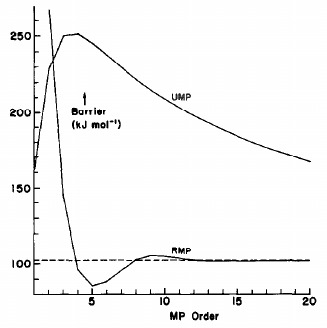
\includegraphics[width=0.45\textwidth]{gill1986.png}
    \caption{\centering Barriers to homolytic fission of \ce{He2^2+} at MPn/STO-3G level ($n = 1$--$20$)\cite{Gill_1986}.}
    \label{fig:my_label}
\end{figure}

When a bond is stretched the exact function can undergo a symmetry breaking becoming multi-reference during this process (see for example the case of \ce{H_2} in \cite{SzaboBook}). A restricted HF Slater determinant is a poor approximation of a broken symmetry wave function but even in the unrestricted formalism, where the spatial orbitals of electrons $\alpha$ and $\beta$ are not restricted to be the same\cite{Fukutome_1981}, which allow a better description of symmetry broken system the series doesn't give accurate results at low orders. Even with this improvement of the zeroth order wave function the series doesn't have the smooth and rapidly converging behavior wanted. 

In the unrestricted framework the ground state singlet wave function is allowed to mix with triplet states which lead to spin contamination. Gill et al. highlighted that there is a link between the slow convergence of the unrestricted MP series and the spin contamination of the wave function as it's shown in the Table 1 within the example of \ce{H_2} in a minimal basis.

\begin{table}[h!]
    \centering
    \begin{tabular}{c c c c c c c}
\hline
 $r$ & UHF & UMP2 & UMP3 & UMP4 & $\expval{S^2}$ \\
\hline
0.75 & 0.0\% & 63.8\% & 87.4\% & 95.9\% & 0.00\\
1.35 & 0.0\% & 15.2\% & 26.1\% & 34.9\% & 0.49\\
2.00 & 0.0\% & 01.0\% & 01.8\% & 02.6\% & 0.95\\
2.50 & 0.0\% & 00.1\% & 00.3\% & 00.4\% & 0.99\\
\hline
\end{tabular}
    \caption{\centering Percentage of electron correlation energy recovered and $\expval{S^2}$ for the \ce{H2} molecule as a function of bond length (r,\si{\angstrom}) in the STO-3G basis set \cite{Gill_1988}.}
    \label{tab:my_label}
\end{table}

Handy and co-workers. exhibited the same behaviors of the series (oscillating and monotonically slowly) in stretched \ce{H_2O} and \ce{NH_2} systems \cite{Handy_1985}. Cremer and He performed the same analysis with 29 FCI systems \cite{Cremer_1996} and regrouped all the systems in two classes. The class A systems which have a monotonic convergence to the FCI value and the class B which converge erratically after initial oscillations. The sample of systems contains stretched molecules and also some at equilibrium geometry, there are also some systems in various basis sets. They highlighted that systems with class A convergence have well-separated electrons pairs whereas class B systems present electrons clustering.

This classification was encouraging in order to develop methods based on perturbation theory as it rationalize the two different convergence modes observed. If it is possible to predict if a system is class A or B, then one can use extrapolation method of the first terms adapted to the class of the systems \cite{Cremer_1996}.

\subsection{Cases of divergence}

But Olsen et al. have discovered even more preoccupying behavior of the MP series in the late 90's. They have shown that the series could be divergent even in systems that they considered as well understood like \ce{Ne} and \ce{HF} \cite{Olsen_1996, Christiansen_1996}. Cremer and He had already studied those two systems and classified them as class B systems. But Olsen and his co-workers have done the analysis in larger basis sets containing diffuse functions and in those basis sets the series become divergent at high order.

\begin{figure}[h!]
    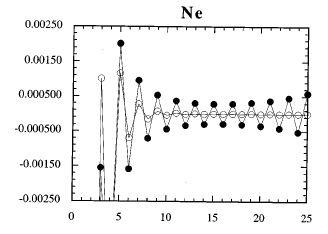
\includegraphics[height=5.5cm]{Nedivergence.png}
    \hfill
    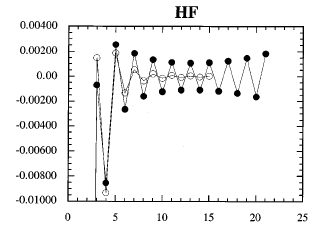
\includegraphics[height=5.5cm]{HFdivergence.png}
    \hfill
    \caption{\centering Correlation contributions for \ce{Ne} and \ce{HF} in the cc-pVTZ-(f/d) $\circ$ and aug-cc-pVDZ $\bullet$ basis sets.}
    \label{fig:my_label}
\end{figure}

The discovery of those divergent behavior was really worrying because in order to get more and more accurate results theoretical chemists need to work in large basis sets. So they investigated the causes of those divergences and in the same time the reasons of the different types of convergence. In order to do this they analyzed the relation between the dominant singularity (i.e. the closest singularity to the origin) and the convergence behavior of the series \cite{Olsen_2000}. Their analysis is based on Darboux's theorem: In the limit of large order, the series coefficients become equivalent to the Taylor series coefficients of the singularity closest to the origin. Following the result of this theorem, one can explain the convergence patterns of the MP series by looking at the dominant singularity

A singularity in the unit circle is designated as an intruder state, more precisely as a front-door (respectively back-door) intruder state if the real part of the singularity is positive (respectively negative). The method used is to do a scan of the real axis to identify the avoided crossing responsible for the pair of dominant singularity. Then by modeling this avoided crossing by a two-state Hamiltonian one can get an approximation of the dominant conjugate pair of singularity by finding the EPs of the 2x2 Hamiltonian. The diagonal matrix is the unperturbed Hamiltonian and the other matrix is the perturbation part of the Hamiltonian.

\begin{equation}
\mqty(\alpha & \delta \\ \delta & \beta) = \mqty(\alpha + \alpha_s & 0 \\ 0 & \beta + \beta_s ) + \mqty(- \alpha_s & \delta \\ \delta & - \beta_s)
\end{equation}
 
They first studied molecules with low-lying doubly excited states of the same spatial and spin symmetry because in those systems the HF wave function is a bad approximation. The exact wave function have non-negligible contribution from the doubly excited states so those low-lying excited states were good candidates for being intruder states. For \ce{CH_2} in a large basis set, the series is convergent up to the 50th order. They have shown that the dominant singularity lies outside the unit circle but close to it causing the slow convergence.

Then they have shown that the divergence for the \ce{Ne} is due to a back-door intruder state. When the basis set is augmented with diffuse functions, the ground state undergo sharp avoided crossings with highly diffuse excited states leading to a back door intruder state. They used their two-state model on this avoided crossings and the model was actually predicting the divergence of the series. They conclude that the divergence of the series was due to the interaction with a highly diffuse excited states. 

Moreover they proved that the extrapolation formula of Cremer and He \cite{Cremer_1996} can't be used for all systems. Even more that those formula were not mathematically motivated when one look at the singularity causing the divergence. For example the hydrogen fluoride molecule contains both back-door intruder states and low-lying doubly excited states which result in alternated terms up to order 10 and then the series is monotonically convergent. This is due to the fact that two pairs of singularity are approximately at the same distance of the origin.

\subsection{The singularity structure}

In the 2000's Sergeev and Goodson \cite{Sergeev_2005, Sergeev_2006}  analyzed this problem from a more mathematical point of view by looking at the whole singularity structure where Olsen and his co-workers were trying to find the dominant singularity causing the divergence. They regroup singularities in two classes: the $\alpha$ singularities which have unit order imaginary parts and the $\beta$ singularities which have very small imaginary parts. The singularities $\alpha$ are related to large avoided crossing between the ground state and a low-lying excited states. Whereas the singularities $\beta$ come from a sharp avoided crossing between the ground state and a highly diffuse state. They succeed to explain the divergence of the series caused by $\beta$ singularities using a previous work of Stillinger \cite{Stillinger_2000}. 

The M{\o}ller-Plesset Hamiltonian is defined as below and by reassembling the term we get the expression (10).

\begin{equation}
H(\lambda)=H_0 + \lambda (H_\text{phys} - H_0)    
\end{equation}

\begin{equation}
    H_\text{phys}=\sum\limits_{j=1}^{n}\left[ -\frac{1}{2}\grad_j^2 - \sum\limits_{k=1}^{N} \frac{Z_k}{|\vb{r}_j-\vb{R}_k|}+\sum\limits_{j<l}^{n}\frac{1}{|\vb{r}_j-\vb{r}_l|}\right]
\end{equation}

\begin{equation}
    H_0=\sum\limits_{j=1}^{n}\left[ -\frac{1}{2}\grad_j^2 - \sum\limits_{k=1}^{N} \frac{Z_k}{|\vb{r}_j-\vb{R}_k|}+V_j^{(scf)}\right]
\end{equation}

\begin{equation}
    H(\lambda)=\sum\limits_{j=1}^{n}\left[-\frac{1}{2}\grad_j^2 - \sum\limits_{k=1}^{N} \frac{Z_k}{|\vb{r}_j-\vb{R}_k|} + (1-\lambda)V_j^{(scf)}+\lambda\sum\limits_{j<l}^{n}\frac{1}{|\vb{r}_j-\vb{r}_l|} \right]
\end{equation}

The first two terms, the kinetic energy and the electron-nucleus attraction, form the mono-electronic core Hamiltonian which is independant of $\lambda$. The third term is the mean field repulsion of the Hartree-Fock calculation done to get $H_0$ and the last term is the Coulomb repulsion. If $\lambda$ is negative, the Coulomb interaction becomes attractive but the mean field stay repulsive as it is proportional to $(1-\lambda)$. If $\lambda$ becomes more and more negative the mean field becomes more and more repulsive so the nucleus can't bind anymore the electrons because the electron-nucleus attraction is not scaled with $\lambda$. But the repulsive mean field is localized around nucleus whereas the electrons interactions persist away from nucleus. So there is a real negative value $\lambda_c$ where the electron form a bound cluster and goes to infinity. According to Baker this value is a critical point of the system and by analogy with thermodynamics the energy $E(\lambda)$ exhibits a singularity at $\lambda_c$. Beyond $\lambda_c$ there is a continuum of eigenstates with electrons dissociated from the nucleus.

This reasoning is done on the exact Hamiltonian and energy, this is the exact energy which exhibits this singularity on the negative real axis. But in finite basis set, one can prove that for a Hermitian Hamiltonian the singularities of $E(\lambda)$ occurs in complex conjugate pair with non-zero imaginary parts. Sergeev and Goodson proved that, as predicted by Stillinger, in a finite basis set the critical point on the real axis modeled by a cluster of sharp avoided crossings with diffuse functions, equivalently by a cluster of $\beta$ singularities in the negative half plane. They explain that Olsen et al., because they used a 2x2 model, only observed the first singularity of this cluster of singularities causing the divergence.

Finally, it has been shown that $\beta$ singularities are very sensitive to the basis sets but not to stretching of the system. On the contrary $\alpha$ singularities are relatively insensitive to the basis sets but very sensitive to bond stretching. According to Goodson the singularity structure from molecules stretched from the equilibrium geometry is difficult \cite{Goodson_2004}, this is conform with the observation of Olsen and co-workers on the \ce{HF} molecule at equilibrium geometry and stretched geometry \cite{Olsen_2000}. To our knowledge the effect of bond stretching on singularities, its link with spin contamination and symmetry breaking of the wave function haven't been as well understood as the ionization effect and its link with diffuse function. In this work we try to improve our understanding of the effect of symmetry breaking on the singularities of $E(\lambda)$ and we hope that it will lead to a deeper understanding of perturbation theory.

\subsection{The physics of quantum phase transition}

%============================================================%
\section{The spherium model}
%============================================================%



\newpage

\bibliographystyle{unsrt}
\bibliography{Rapport}



\end{document}
